% Created 2020-03-05 Thu 13:08
% Intended LaTeX compiler: pdflatex
\documentclass[a4paper]{article}

\usepackage{booktabs}
\usepackage[margin=2cm]{geometry}
\usepackage{sourcecodepro}
\usepackage{booktabs}
\usepackage{array}
\usepackage{colortbl}
\usepackage{listings}
\usepackage{algpseudocode}
\usepackage{algorithm}
\usepackage{graphicx}
\usepackage[english]{babel}
\usepackage[scale=2]{ccicons}
\usepackage{hyperref}
\usepackage{relsize}
\usepackage{amsmath}
\usepackage{bm}
\usepackage{amsfonts}
\usepackage{wasysym}
\usepackage{float}
\usepackage{ragged2e}
\usepackage{textcomp}
\usepackage{pgfplots}
\usepackage{todonotes}
\usepgfplotslibrary{dateplot}
\lstdefinelanguage{Julia}%
{morekeywords={abstract,struct,break,case,catch,const,continue,do,else,elseif,%
end,export,false,for,function,immutable,mutable,using,import,importall,if,in,%
macro,module,quote,return,switch,true,try,catch,type,typealias,%
while,<:,+,-,::,/},%
sensitive=true,%
alsoother={$},%
morecomment=[l]\#,%
morecomment=[n]{\#=}{=\#},%
morestring=[s]{"}{"},%
morestring=[m]{'}{'},%
}[keywords,comments,strings]%
\lstset{ %
backgroundcolor={},
basicstyle=\ttfamily\scriptsize,
breakatwhitespace=true,
breaklines=true,
captionpos=n,
extendedchars=true,
frame=n,
language=R,
rulecolor=\color{black},
showspaces=false,
showstringspaces=false,
showtabs=false,
stepnumber=2,
stringstyle=\color{gray},
tabsize=2,
}
\renewcommand*{\UrlFont}{\ttfamily\smaller\relax}
\author{Pedro Bruel}
\date{\today}
\title{Mean Performance with Varying Injection Rate}
\hypersetup{
 pdfauthor={Pedro Bruel},
 pdftitle={Mean Performance with Varying Injection Rate},
 pdfkeywords={},
 pdfsubject={},
 pdfcreator={Emacs 26.3 (Org mode 9.2.5)},
 pdflang={English}}
\begin{document}

\maketitle
The experiment  consists of changing  injection rates  \(inj_1\) and \(inj_2\),  for 2
applications in  Supersim, and optimize the  execution times \(\mathcal{P}(inj_1)\)
and \(\mathcal{P}(inj_2)\).  The experimental settings are:

\begin{center}
\begin{tabular}{ll}
\hline
Parameter & Value\\
\hline
Injection Rate 1 (\(inj_1\)) & \([0.1, 0.5]\)\\
Injection Rate 2 (\(inj_2\)) & \([0.1, 0.5]\)\\
Performance Metric & \(\frac{\mathcal{P}_1(inj_1) + \mathcal{P}_2(inj_2)}{2}\)\\
\hline
\end{tabular}
\end{center}

The interval for  injection rates was limited because the  simulator crashed for
larger rates.   The problem must  be better  understood to determine  the proper
injection rate ranges.

Low-discrepancy samples  of size 20 were  taken for both injection  rates on the
specified intervals,  and 10 repetitions  were performed. In total,  200 samples
were measured, and the best value according to the performance metric was logged
separately for each repetition.

\section{Results with Average of Execution Times}
\label{sec:orgd8e077e}
The figure  below shows the injection  rates, for both applications,  in the 200
samples tested.

\begin{center}
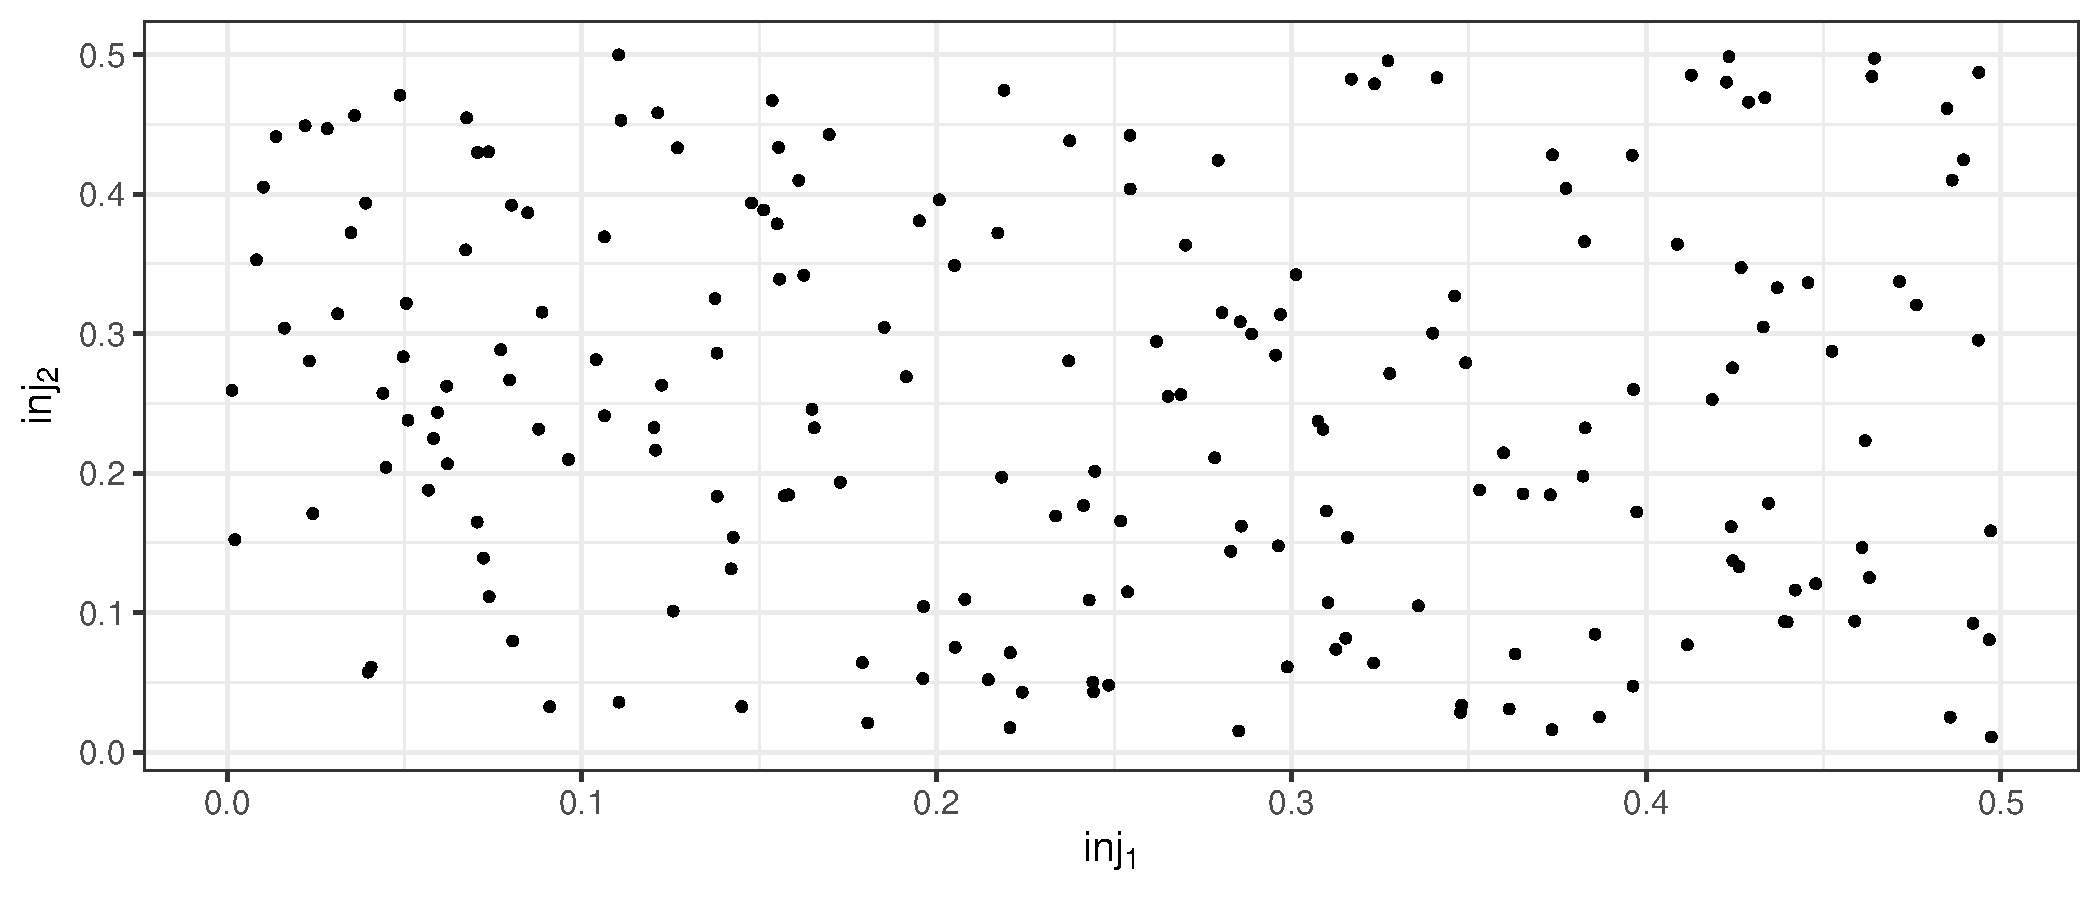
\includegraphics[width=0.8\textwidth]{./img/2_apps_min_mean_time/rs_20_samples_10_iterations_injection_scatter.pdf}
\end{center}

\subsection{Histograms}
\label{sec:orgbe15910}
Looking at the  histograms of the performance metric and  the execution times of
both  applications,  in  the  figure  below,  we see  that  almost  150  of  the
configurations tested had performance below \(10^{9}\).

\begin{center}
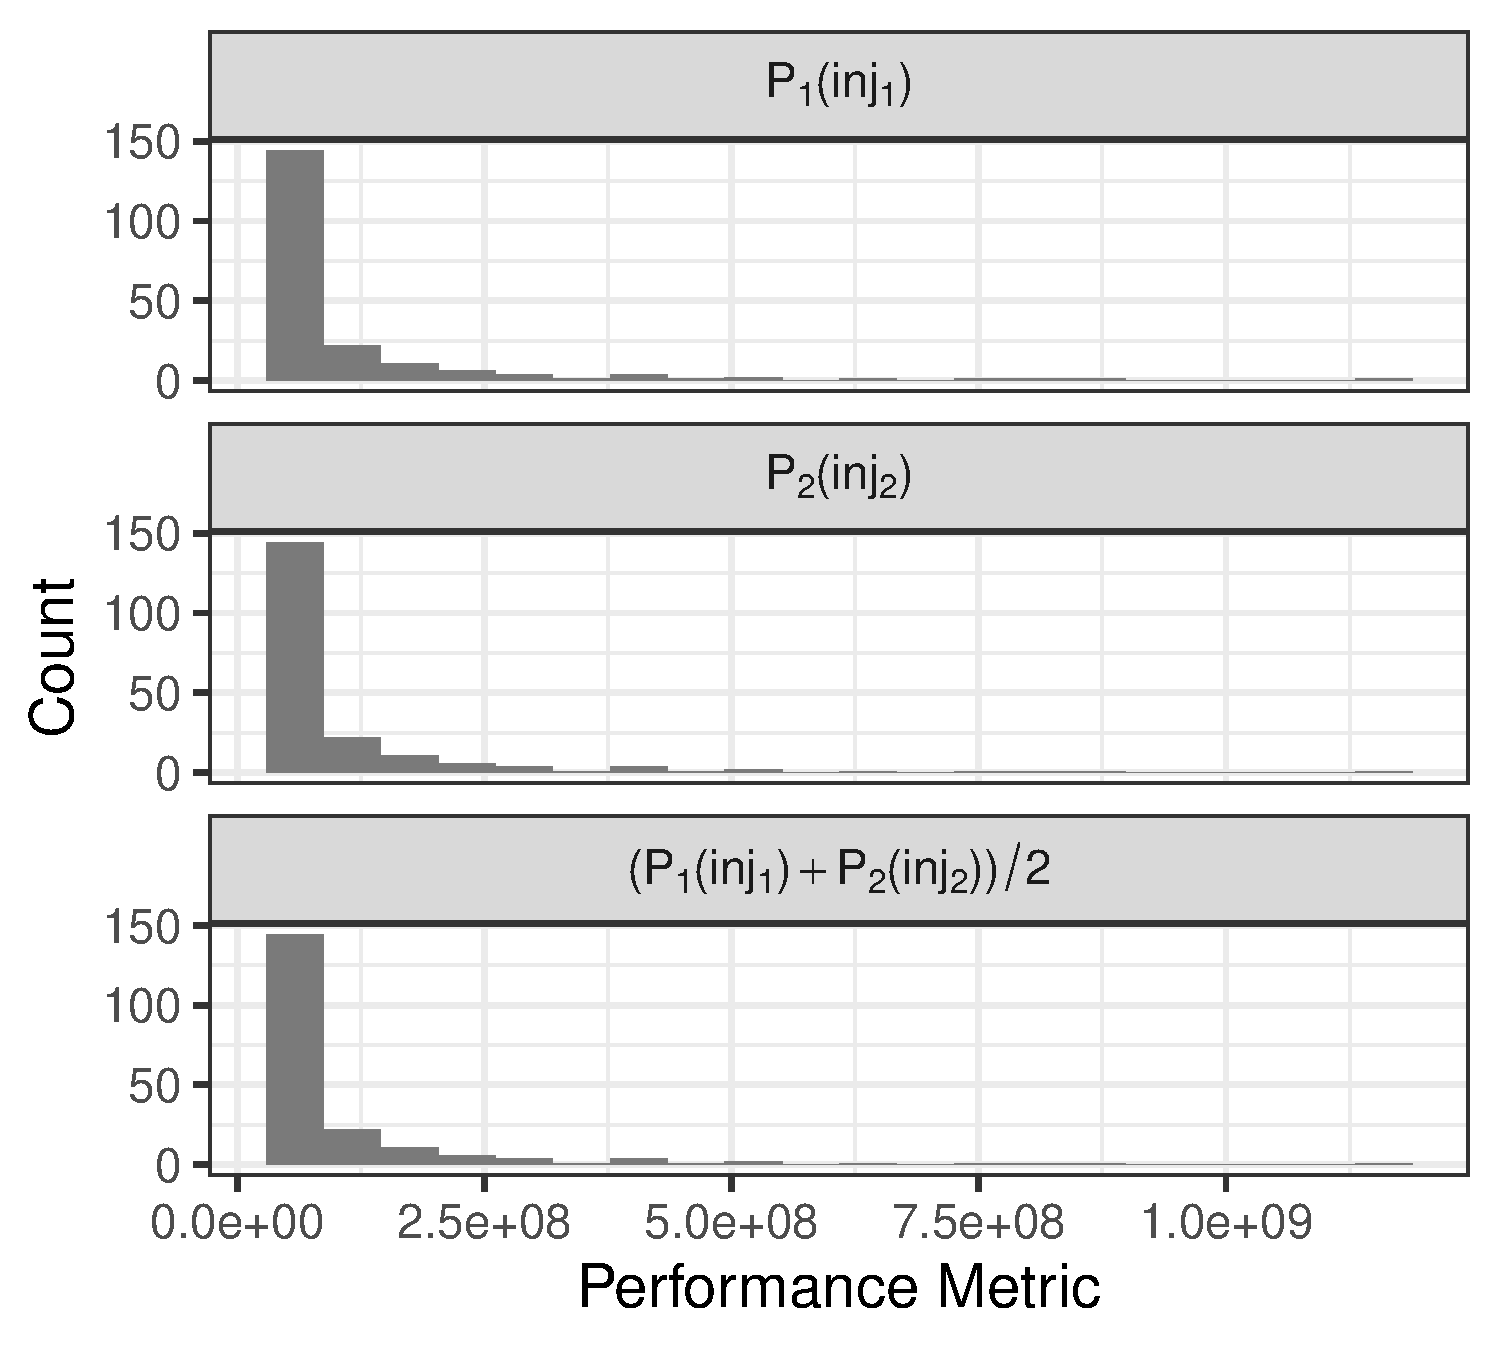
\includegraphics[width=0.5\textwidth]{./img/2_apps_min_mean_time/rs_20_samples_10_iterations_histogram.pdf}
\end{center}

Below, we take a closer look at the lower end performance measurements.

\begin{center}
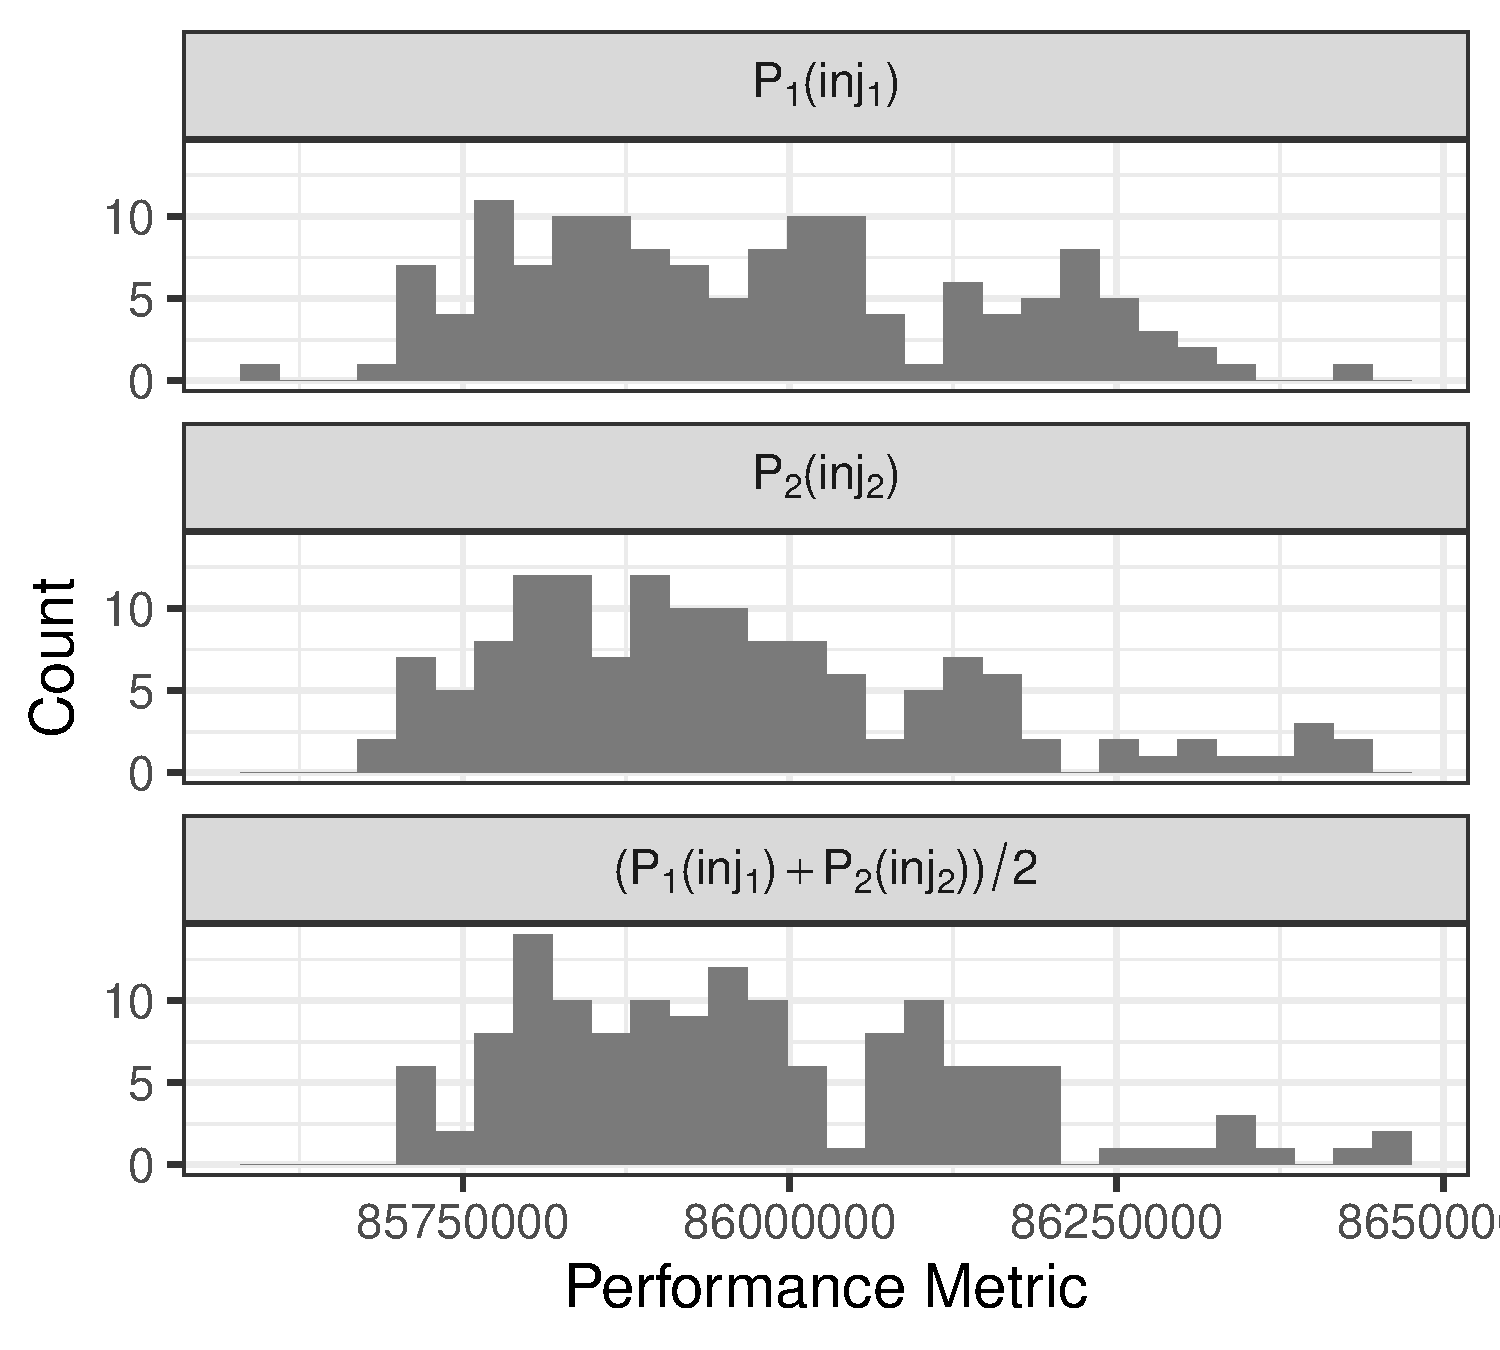
\includegraphics[width=0.5\textwidth]{./img/2_apps_min_mean_time/rs_20_samples_10_iterations_histogram_cut.pdf}
\end{center}

\subsection{Mean Performance and Injection Rate}
\label{sec:orgd50c907}
We  now  look  at  the  performance metric  measured  for  each  injection  rate
configuration.  The  figure below splits the  values of injection rate  for each
application, and shows the performance metric computed using the execution times
of both applications.

\begin{center}
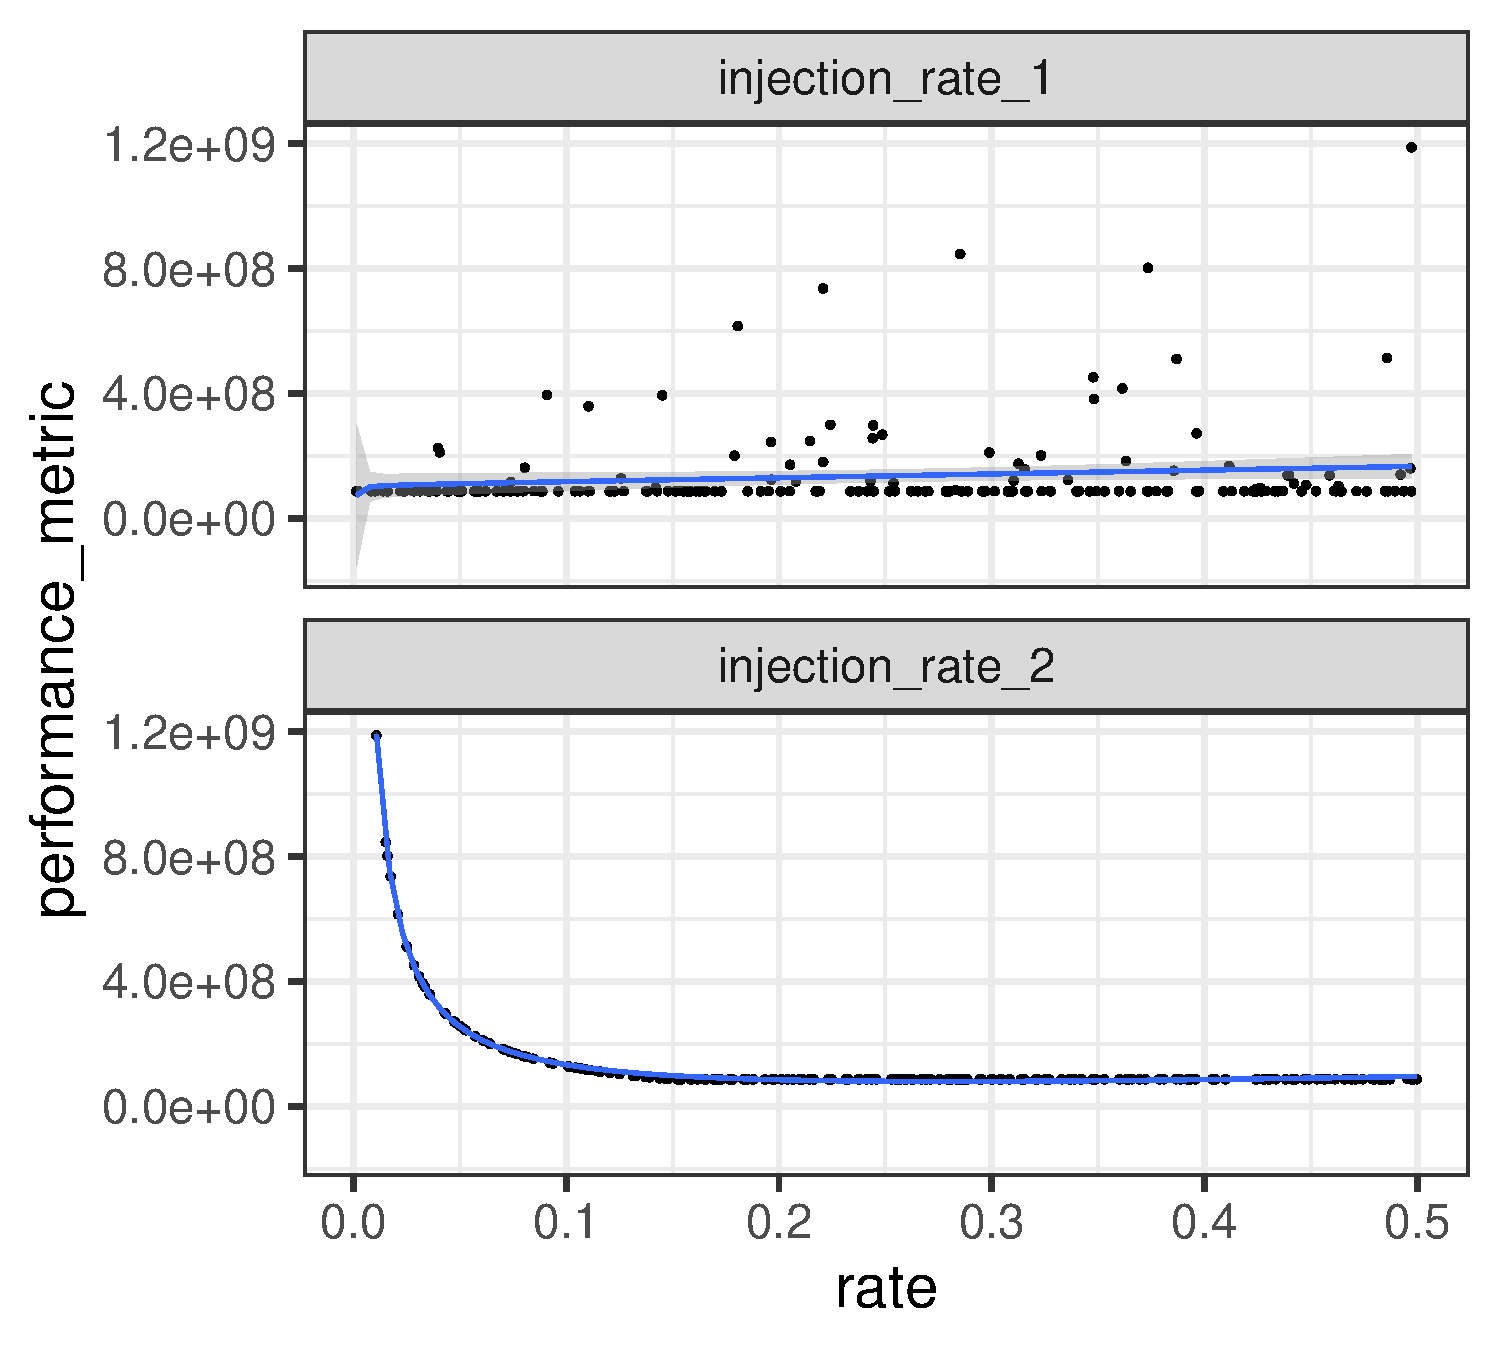
\includegraphics[width=0.6\textwidth]{./img/2_apps_min_mean_time/rs_20_samples_10_iterations_scatter.pdf}
\end{center}

The solid lines represent the fit of the collected data to the linear models
\begin{equation*}
\dfrac{\mathcal{P}(inj_1) + \mathcal{P}(inj_2)}{2} =
Y_1 = \beta_{1}inj_1 +
\beta_{2}\left(\dfrac{1}{inj_1}\right)\text{,}
\end{equation*}
for the top box, and
\begin{equation*}
\dfrac{\mathcal{P}(inj_1) + \mathcal{P}(inj_2)}{2} =
Y_2 = \beta_{3}inj_2 +
\beta_{4}\left(\dfrac{1}{inj_2}\right)\text{,}
\end{equation*}
for the bottom box. The shaded  regions represent the 95\% confidence interval of
the mean.

Visual inspection of  these fits indicates that \(inj_1\) does  not affect the mean
performance metric  as much as  \(inj_2\), which also have  a strong effect  in the
performance of application  1. The mean performance metric seems  to fit well to
the model using \(inj_2\).

\subsection{ANOVA and Linear Model Fit}
\label{sec:orgf99dab2}
We  now perform  statistical  tests  to confirm  the  visual  analyses from  the
previous section.   We perform a  linear model fit using  the 20 samples  from a
single experiment, picked  at random between the 10  repetitions performed.  The
linear model we have used was
\begin{equation*}
\dfrac{\mathcal{P}(inj_1) + \mathcal{P}(inj_2)}{2} =
Y = \beta_{1}inj_1 +
\beta_{2}inj_2 +
\beta_{3}\left(\dfrac{1}{inj_1}\right) +
\beta_{4}\left(\dfrac{1}{inj_2}\right) +
\beta_{5}\left(inj_{1}inj_{2}\right) +
\beta_{6}\left(\dfrac{1}{inj_{1}inj_2}\right)\text{.}
\end{equation*}


% latex table generated in R 3.6.3 by xtable 1.8-4 package
% Thu Mar  5 12:36:02 2020
\begin{table}[ht]
\centering
\caption{Regression coefficients for a linear model fit using 20 experiments}
\begin{tabular}{lrr}
  \toprule
Model Term & Coefficient & Significance p-value \\
  \midrule
Intercept & $8.4 \times 10^{6}$ & $5.1 \times 10^{-1}$ \\
  injection\_rate\_1 & $-6.6 \times 10^{7}$ & $1.1 \times 10^{-1}$ \\
  injection\_rate\_2 & $1.1 \times 10^{8}$ & $1.0 \times 10^{-2}$ \\
  1/injection\_rate\_1 & $2.9 \times 10^{5}$ & $5.9 \times 10^{-1}$ \\
  1/injection\_rate\_2 & $1.4 \times 10^{7}$ & $3.0 \times 10^{-13}$ \\
  injection\_rate\_1 $\times$ injection\_rate\_2 & $1.7 \times 10^{8}$ & $1.6 \times 10^{-1}$ \\
  1/injection\_rate\_1 $\times$ 1/injection\_rate\_2 & $-1.9 \times 10^{5}$ & $1.2 \times 10^{-1}$ \\
   \bottomrule
\end{tabular}
\end{table}

The  model coefficient  magnitude and  significance values  confirm that  \(inj_2\)
impacts the mean performance more than \(inj_1\), and the interaction between these
factors seem to not be significant  in this experiment. We also perform analysis
of variance,  using the same  performance mode,  for a single  20-run experiment
picked at random, shown in the table below.


% latex table generated in R 3.6.3 by xtable 1.8-4 package
% Thu Mar  5 12:37:13 2020
\begin{table}[ht]
\centering
\caption{Analisys of variance for a linear model fit using 20 experiments}
\begin{tabular}{lr}
  \toprule
Model Term & Significance p-value \\
  \midrule
injection\_rate\_1 & $4.4 \times 10^{-9}$ \\
  injection\_rate\_2 & $1.1 \times 10^{-18}$ \\
  1/injection\_rate\_1 & $1.5 \times 10^{-5}$ \\
  1/injection\_rate\_2 & $6.8 \times 10^{-20}$ \\
  injection\_rate\_1 $\times$ injection\_rate\_2 & $9.0 \times 10^{-1}$ \\
  1/injection\_rate\_1 $\times$ 1/injection\_rate\_2 & $5.4 \times 10^{-1}$ \\
  Residuals &  \\
   \bottomrule
\end{tabular}
\end{table}

We see again that  the terms using \(inj_2\) explain more  of the observed variance
on the performance metric. For further experiments using these two applications,
performance mean can be modeled and minimized using only a linear and an inverse
term  for  \(inj_2\).  Further  steps   should  be  attempting  to  generalize  the
statistical analysis  for more applications  running at  the same time,  or with
more controllable parameters.
\end{document}
